\begin{figure}[ht]
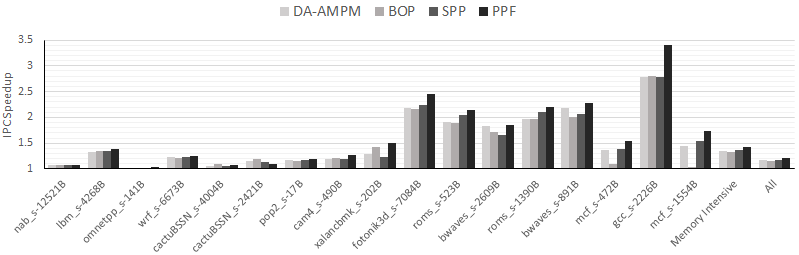
\includegraphics[width=\columnwidth]{SPEC2017}
\caption{SPEC 2017 Single-Core IPC Speedup}
\label{Fig:SPEC2017_1core}
\end{figure}

\section{Results}
\label{Results}

This section discusses the results obtained from running PPF, in
terms of prefetch cache coverage and Instruction Per
Cycle (IPC).  For SPEC 2017 suite, first we present the
results for single-threaded workloads then for multi-core
workloads.

\subsection{Single-core Results}
\label{Results-Single}


Figure~\ref{Fig:SPEC2017_1core} shows the IPC speedup obtained by
PPF, compared to BOP, DA-AMPM and SPP. 
In the figure we have depicted selected traces, where PPF shows a 
noticeable improvement or shows some degradation, along with the 
geometric mean improvement on the memory intensive subset of SPEC 2017, 
and finally for the complete SPEC 2017 benchmark. 
All the results have been normalized to baseline \textit{i.e.}, no
prefetching.  

As can be seen, PPF yields a speedup of \textbf{42.8\%} over
the baseline. This is equivalent to \textbf{7.8\%} over DA-AMPM, \textbf{9.7\%} over BOP
and \textbf{6.92\%} over SPP.  Out of the 95 simpoints developed for SPEC 2017, 
PPF nearly matches or outperforms most of the prefetchers on 91 simpoints.
Only in 607.cactuBSSN and 654.roms, PPF fails to match the improvement 
offered by BOP.

At its peak, PPF manages to get the IPC speedup of a factor of
over \textbf{3.39x} on the trace \textit{602.gcc\_s-2226B}.  This also
corresponds to speedup gain of \textbf{60\%} over the next best
prefetcher -- BOP. 
In general, benchmarks \textit{bwaves, mcf, xalancbmk} 
and \textit{fotonik3d} benefit the most from PPF, with the speedup over
SPP ranging from \textbf{10\% to 25\%}.

On the full SPEC 2017 suite, PPF improves the baseline by \textbf{20.9\%},
which is \textbf{3.44\%} more than the next best prefetcher -- SPP.

\begin{figure}[h]
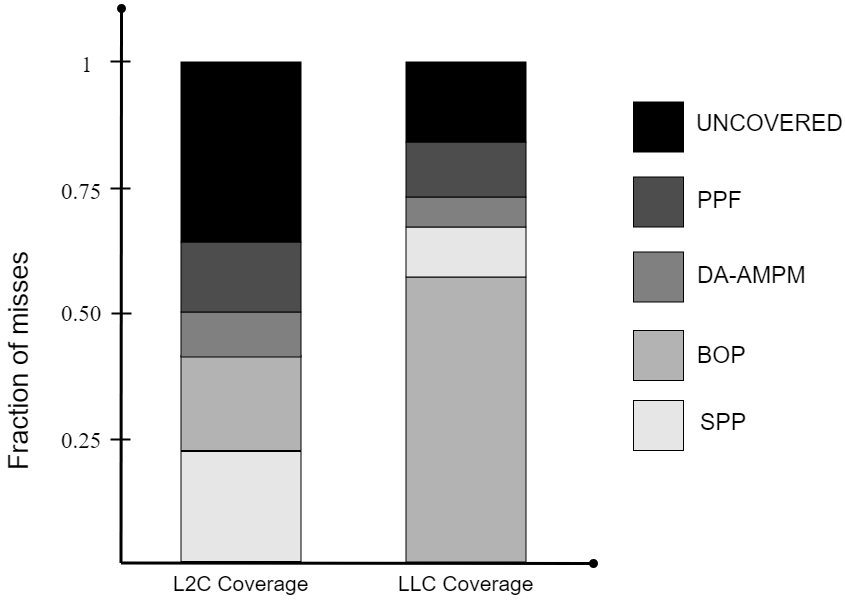
\includegraphics[width=\columnwidth]{Coverage}
\caption{Fraction of Cache Misses Covered}
\label{Fig:Coverage}
\end{figure}

\textbf{Coverage}\newline
A prefetcher coverage can be defined as the ratio of number of misses 
avoided through prefetching to the number of misses in presence of no 
prefetchig.
Figure~\ref{Fig:Coverage} shows the fraction of misses in L2 and Last
Level Caches avoided by the various prefetchers.
PPF has the highest coverage of all the prefetchers simulated. Using PPF 
on SPEC 2017 benchmark, 
misses can be reduced by \textbf{62.5\%} and \textbf{82.8\%} in L2 Cache and Last Level 
Cache respectively. For the same benchmark, the next best prefetcher -- 
DA-AMPM covers \textbf{48.6\%} and \textbf{72.8\%} of the misses respectively.

This superior coverage of PPF can be attributed to aggressive 
re-tuning of the underlying SPP. At the same time, the Perceptron Filter
makes sure than this high coverage does not lead to an increased 
cache pollution. 


\begin{figure}[h]
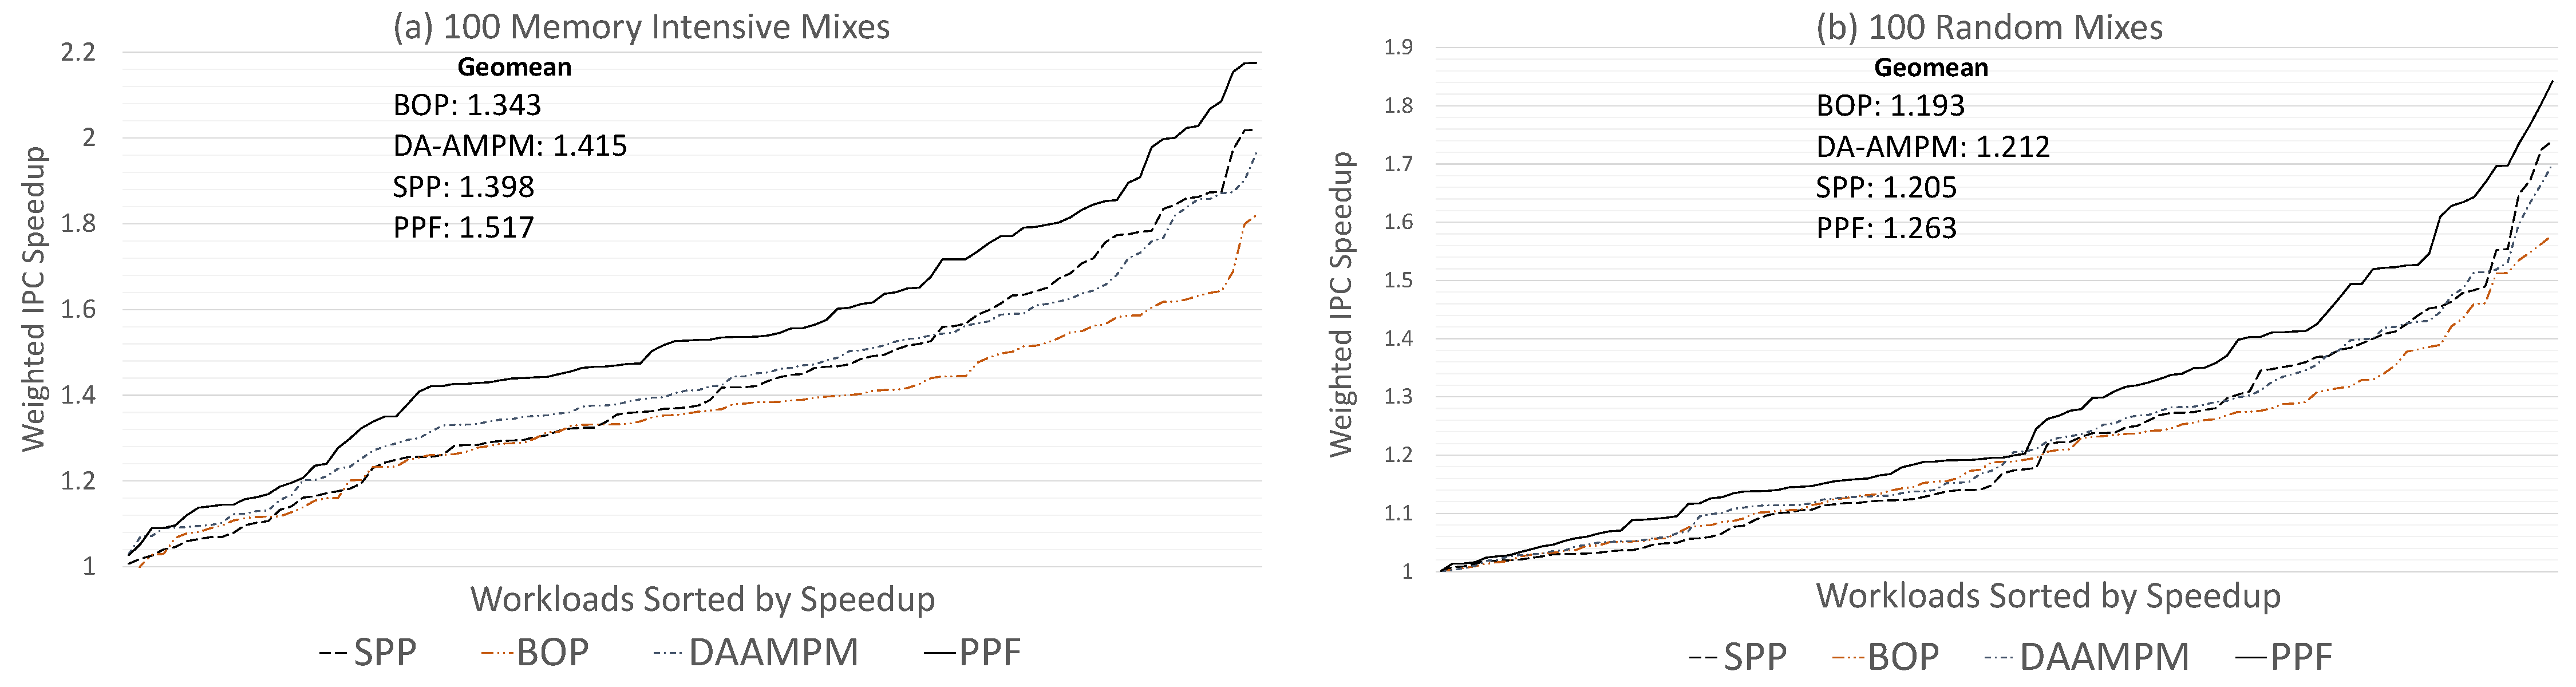
\includegraphics[width=\columnwidth]{4Core_SPEC2017}
\caption{Normalized speedup for 4-core workloads}
\label{Fig:4Core_SPEC2017}
\end{figure}


\subsection{Multi-core Results}
\label{Results-Multi}
In this section, we demonstrate the improvement achieved by PPF
for a mix of multi-programmed workloads.

\textit{4-core environment} Figure~\ref{Fig:4Core_SPEC2017} (a) 
shows a comparison of speedups
obtained on 4-core mix of memory intensive subset of SPEC 2017.  We
plot all the 4 prefetchers, normalized to the baseline.  The workloads
have been sorted in the increasing order of the speedup.
As can be seen,
PPF offers an IPC improvement by \textbf{51.7\%} on these traces.  
Compared to the base prefetcher -- SPP only, this is \textbf{11.9\%} more.
As compared to the next best prefetcher -- DA-AMPM, this is 
This is \textbf{10.2\%} and \textbf{17.4\%} over DA-AMPM, 
the next best prefetcher, and BOP, respectively.

On a different set of fully random SPEC 2017 4-core mixes, 
PPF provides an IPC speedup of 
\textbf{26.2}\% over baseline, which is \textbf{5.7}\% more than just SPP.


\begin{figure}[h]
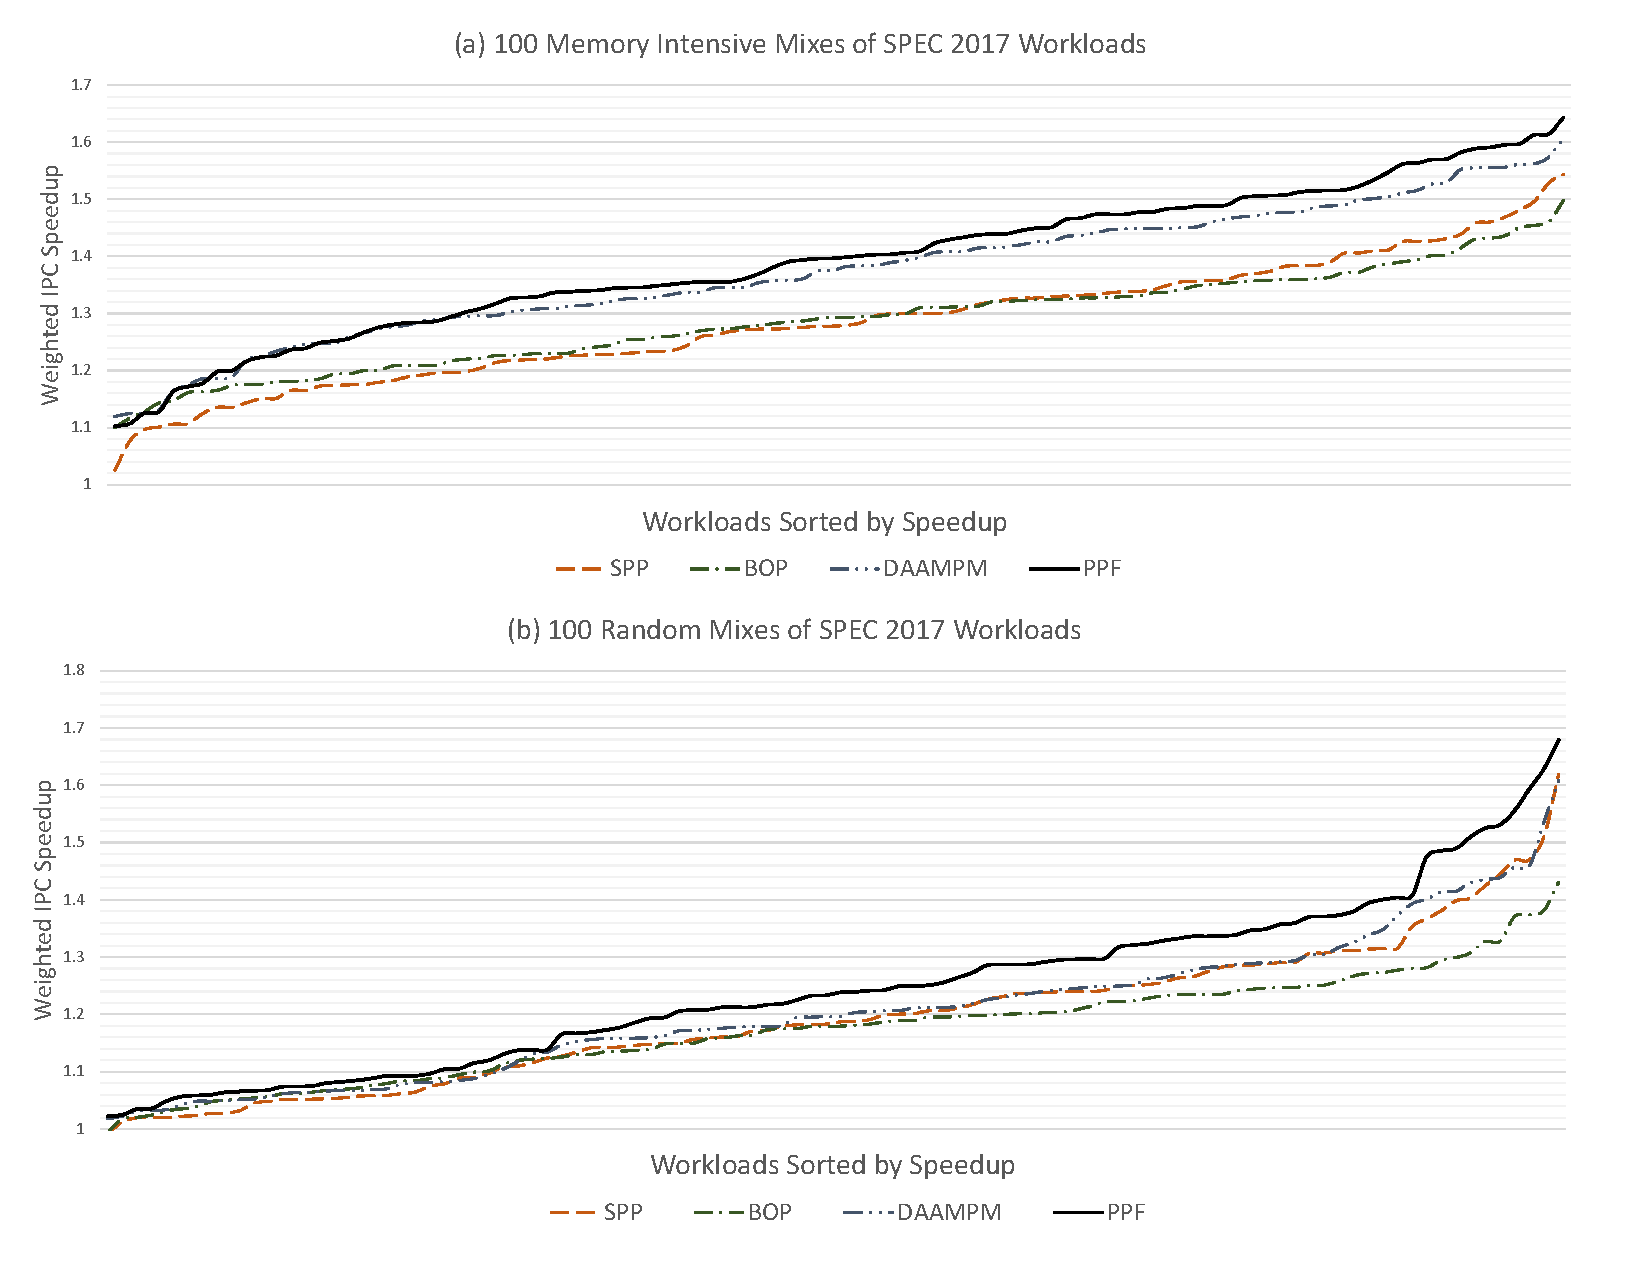
\includegraphics[width=\columnwidth]{8Core_SPEC2017}
\caption{Normalized speedup for 8-core workloads}
\label{Fig:8Core_SPEC2017}
\end{figure}


\textit{8-core environment} The sorted comparison of speedup obtained 
on the memory intensive 8-core mixes is depicted in Fig~\ref{Fig:8Core_SPEC2017}.
PPF improves baseline performance by \textbf{38.6\%} and that is \textbf{10.7\%} 
more than using just SPP. 
For completely random set of SPEC 2017 mixes, PPF improves performance by 
\textbf{23.6\%} over the baseline, corresponding to \textbf{4.8\%} over SPP.
This increased improvement achieved by PPF over the base engine SPP,
in a multi-core environment is not surprising. 
Since PPF has an extremely intelligent filter, it ends up 
eliminating useless prefetches before they can create cache
pollution in the shared LLC. 

As can be seen, BOP offer a better improvement than 
SPP, for the memory intensive mix, This can be attributed 
to BOP's inherent aggressive nature. DA-AMPM is also ahead of
SPP in both the mixes. Interestingly, in all these cases, 
PPF consistently outperforms the best performing prefetcher.

%[EB] How to justify only a small margin over DA-AMPM?

\begin{figure}[ht]
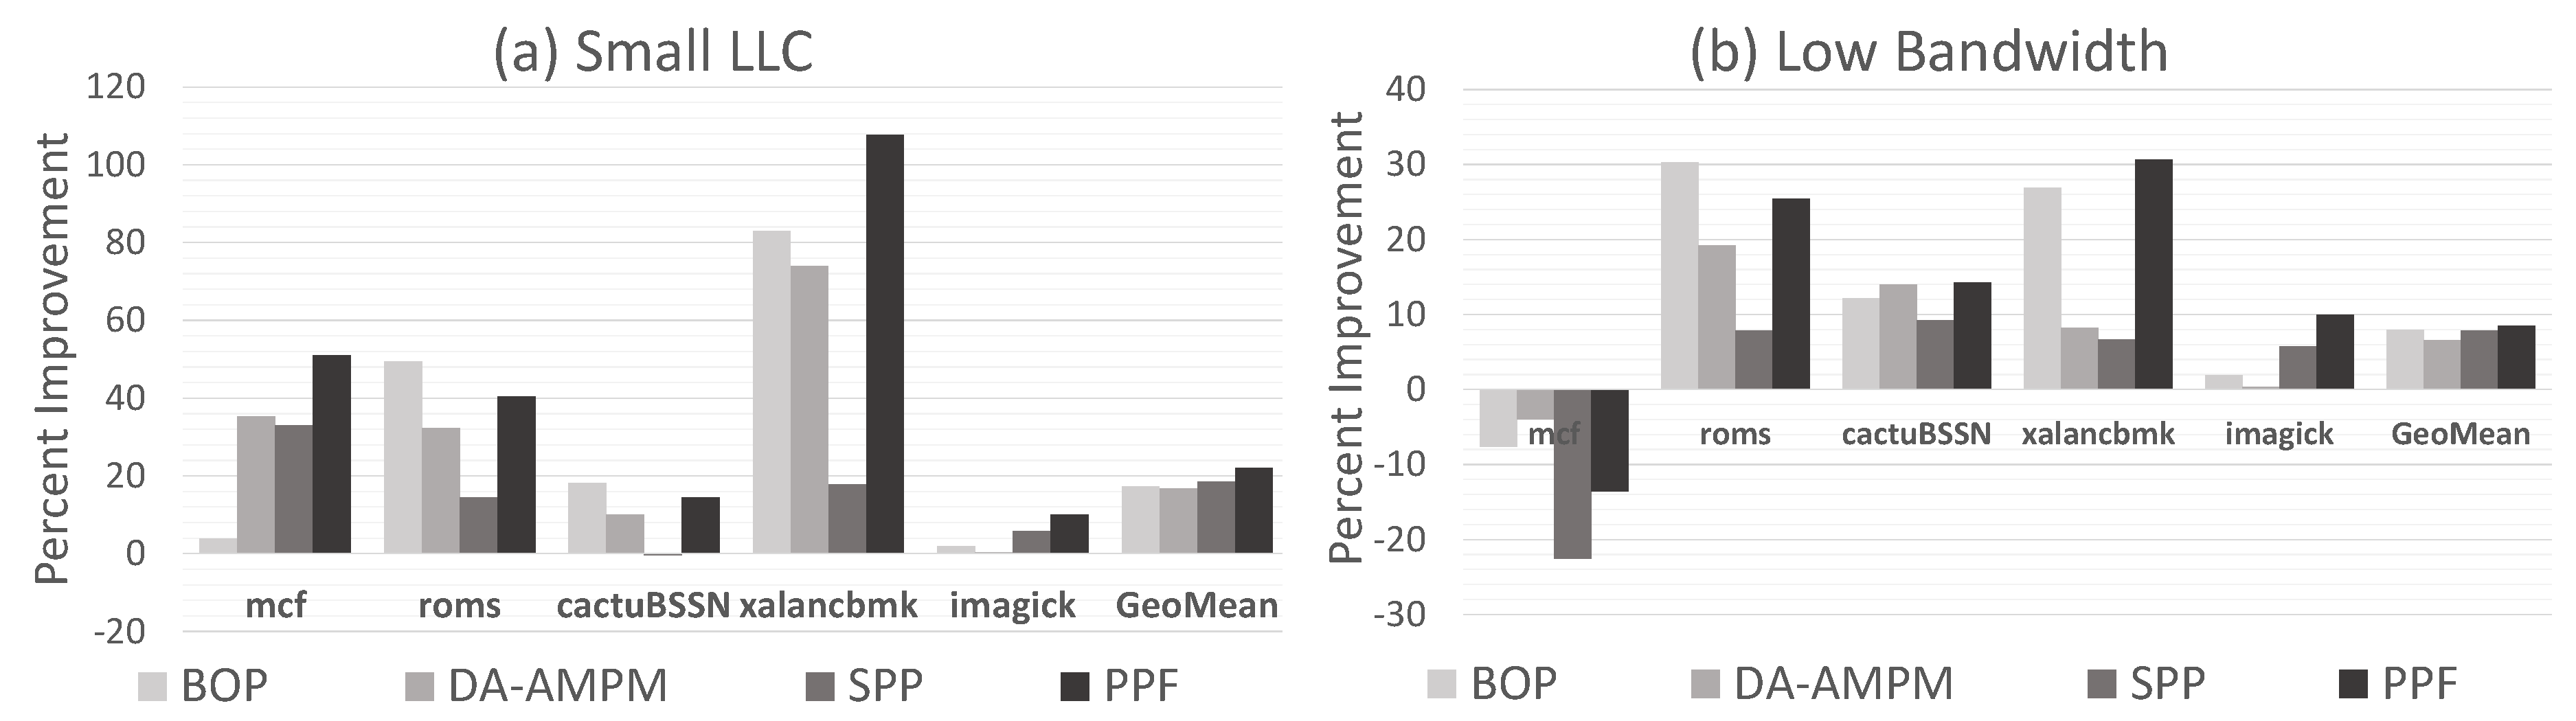
\includegraphics[width=\columnwidth]{AddnConstr}
\caption{IPC speedup for Small LLC and Low BW}
\label{Fig:AddnConstr}
\end{figure}

\subsection{Additional Memory Constraints}
\label{Results-AdditionalMem}

Figure \ref{Fig:AddnConstr}(a) and (b) show the performance of PPF in a 
reduced LLC and low bandwidth constraints respectively. For the sake of brevity, 
we have only shownselected traces, followed
by the overall performance on the complete benchmark.
As can be seen, \textit{mcf} in low bandwidth conditions is prefetch averse.
In general, any prefetcher yields a negative speedup on that trace.
On \textit{roms} and \textit{cactuBSSN}, PPF is unable to match the performance 
achieved by the best prefetcher. On the other hand, PPF outperforms all the 
other prefetchers on \textit{xalancbmk} and \textit{imagick} benchmarks.
Overall, PPF gives a better improvement under small LLC condition and 
matches the best prefetcher -- BOP under low DRAM bandwidth condition.

\begin{figure}[ht]
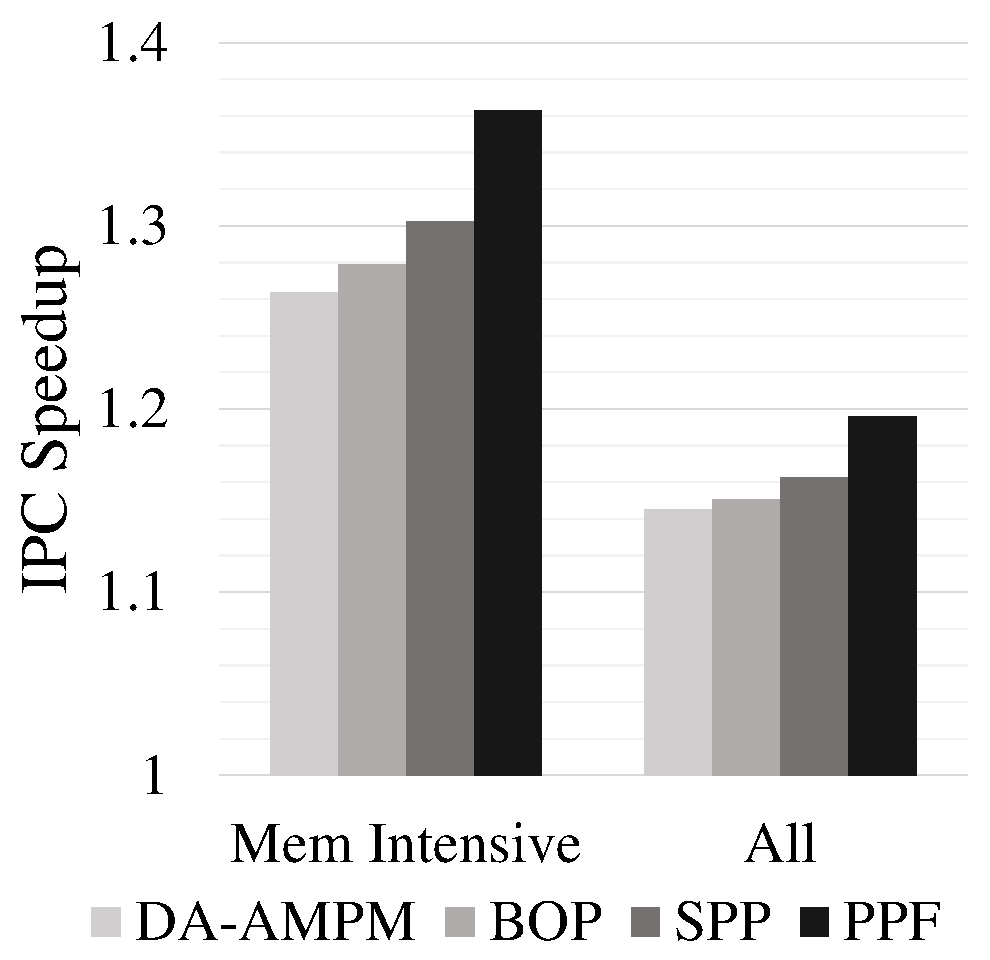
\includegraphics[width=\columnwidth]{SPEC2006}
\caption{SPEC 2006 Single-Core IPC Speedup}
\label{Fig:SPEC2006_1core}
\end{figure}

\begin{figure}[ht]
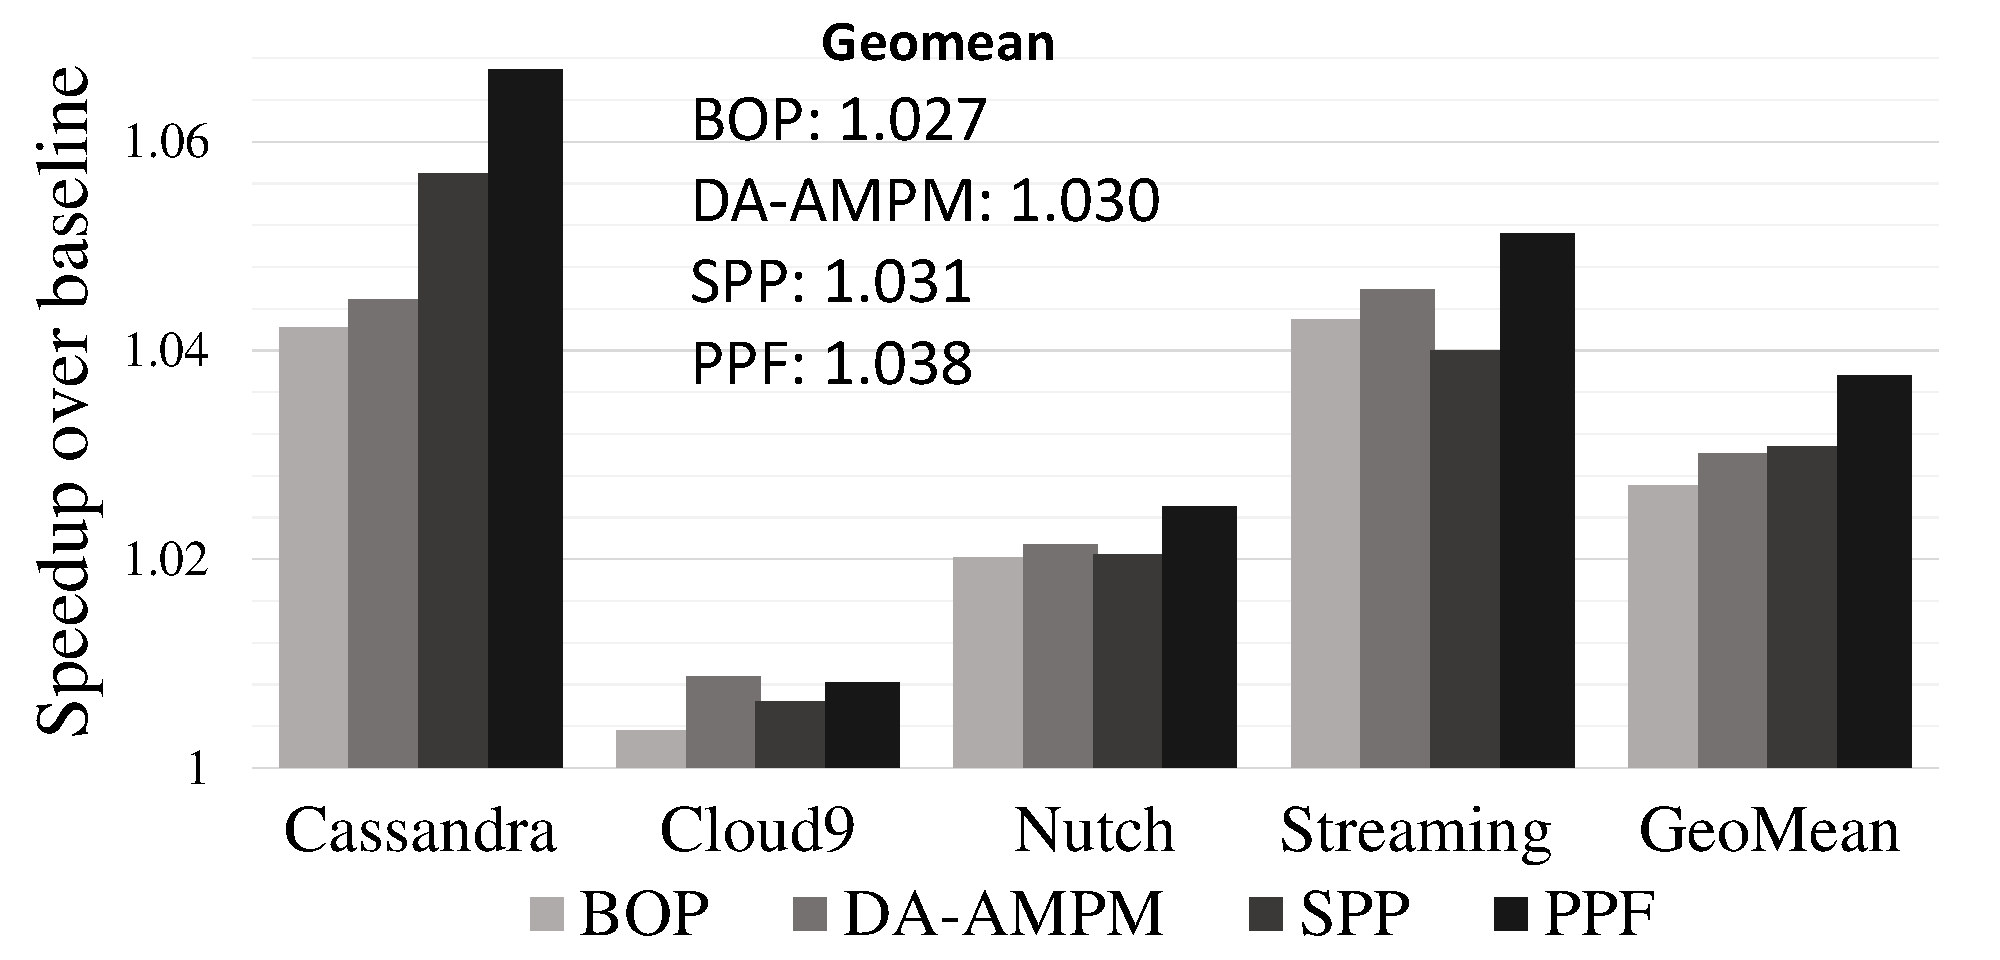
\includegraphics[width=\columnwidth,]{CloudSuite}
\caption{IPC Speedup for Multi-core CloudSuite Workloads}
\label{Fig:CloudSuite}
\end{figure}

\subsection{Cross Validation}
\label{Results-CrossVal}

Here we try to demonstrate the robustness of PPF by testing it on
completely unseen benchmarks, namely SPEC 2006 and CloudSuite.

Fig~\ref{Fig:SPEC2006_1core} shows the speed-up achieved by BOP, SPP and PPF on
selected traces of SPEC 2006, along with the overall geometric mean
over whole of the benchmark and over memory-intensive subset of the
SPEC 2006 benchmark.  As can be seen, PPF provides a speed-up of
\textbf{46.1\%} over baseline, on the memory intensive subset of SPEC 2006
benchmark. This corresponds to \textbf{6.66\%} over SPP and \textbf{9.86\%} over BOP and DA-AMPM.  
On the whole of the SPEC 2006 suite, the speedup obtained is \textbf{22.4\%},
which is \textbf{3.34\%} ahead of SPP.

For 4-core memory intensive mixes, PPF improves the baseline by \textbf{59.2\%}, 
\textbf{8.7\%} ahead of SPP. For 8-core memory intensive mixes, the IPC speedup 
over baseline is \textbf{47.9\%}, \textbf{11.5\%} ahead of SPP. 

Figure~\ref{Fig:CloudSuite} shows the performance benefit comparison of all 
the prefetch schemes on 4 different applications in the CloudSuite benchmark. 
In general, these applications are prefetch agnostic. Even in that scenario, 
PPF manages a \textbf{3.7\%} improvement over no prefetching, making it ahead of the 
next best prefetcher -- SPP, which provides a 3.08\% IPC speedup.

As can be seen, the performance is very consistent given no prior
parameter tuning was done keeping these benchmarks in mind.  We attribute
this to the inherent adaptability of the perceptron model.  In
general, perceptron weights are able to adjust in real-time so as to
find the best possible correlation between the output and the given set of 
features.
